\subsection{Overview}

The survey below was written to understand the aspects of the different programs that are similar and different from the Reggio Approach. This survey was used to structure interviews with administrators and educators in the different school systems in Reggio Emilia, Parma, and Padova. We summarize the components of the Reggio Approach below.

\begin{itemize}
\item Administrative components
\begin{itemize}
	\item Full-time educative coordinators, with a university degree in psychology or education, were hired by the school system.
	\item Educative coordinators met biweekly with educative staff to provide mentoring and professional development.
	\item Kitchen staff participated in professional development and routine trainings with teachers.
	\item Support staff participated in professional development and routine trainings with teachers.
	\item Teachers participated in professional development with teachers from other school systems (e.g. municipal and private Catholic).
	\item Schools were open daily for 8 hours.
	\item Schools offered extended hours for working families.
	\item Scheduled work hours are set aside weekly for teachers to engage families.
	\item Scheduled work hours are set aside weekly for teachers to document children's work.
	\item Scheduled work hours are set aside weekly for teachers to participate in professional development.
	\item Priority of enrollment is given to economically disadvantaged families.
	\item Priority of enrollment is given to single-parent families.
	\item Priority of enrollment is given to children with disabilities.
	\item Schools received funding from public sources. 
\end{itemize}
\item Pedagogical components
\begin{itemize}
	\item Daily activities were implemented by following a program to guide children in acquiring knowledge of specific concepts.
	\item Classrooms were homogenous in age.
	\item Two co-teachers were assigned to the same group of children. Continuity of care provided by keeping at least one teacher with the same group from year to year.
	\item A full-time, on-site teacher with specific training or experience in the fine arts helped educators design creative learning activities.
	\item Visual arts were used as a tool to help children learn.
	\item Children receive religious teaching.
	\item Teachers keep a record of children's learning.
	\item The design of the school environment emphasizes open spaces, natural lighting, and the use of natural materials for furniture.
	\item The school environment included a dedicated room where children from different classrooms work individually or in small groups.
	\item An on-site kitchen was used daily to prepare meals. \textbf{We omit this characteristic.}
	\item Unlimited project timelines shaped the educational program.
	\item Academic theories of psychology and early childhood education influenced educational approaches.
	\item Early childhood methodologies endorsed influenced the daily program.
	\item Educational practices promoted by Loris Malaguzzi for early childhood influenced the daily program.
	\item The educational program is designed to promote good morals of family life, and is based on love of family and the homeland.
	\item Parental boards or advisory groups were encouraged and active participants in school culture.
\end{itemize}
\end{itemize}

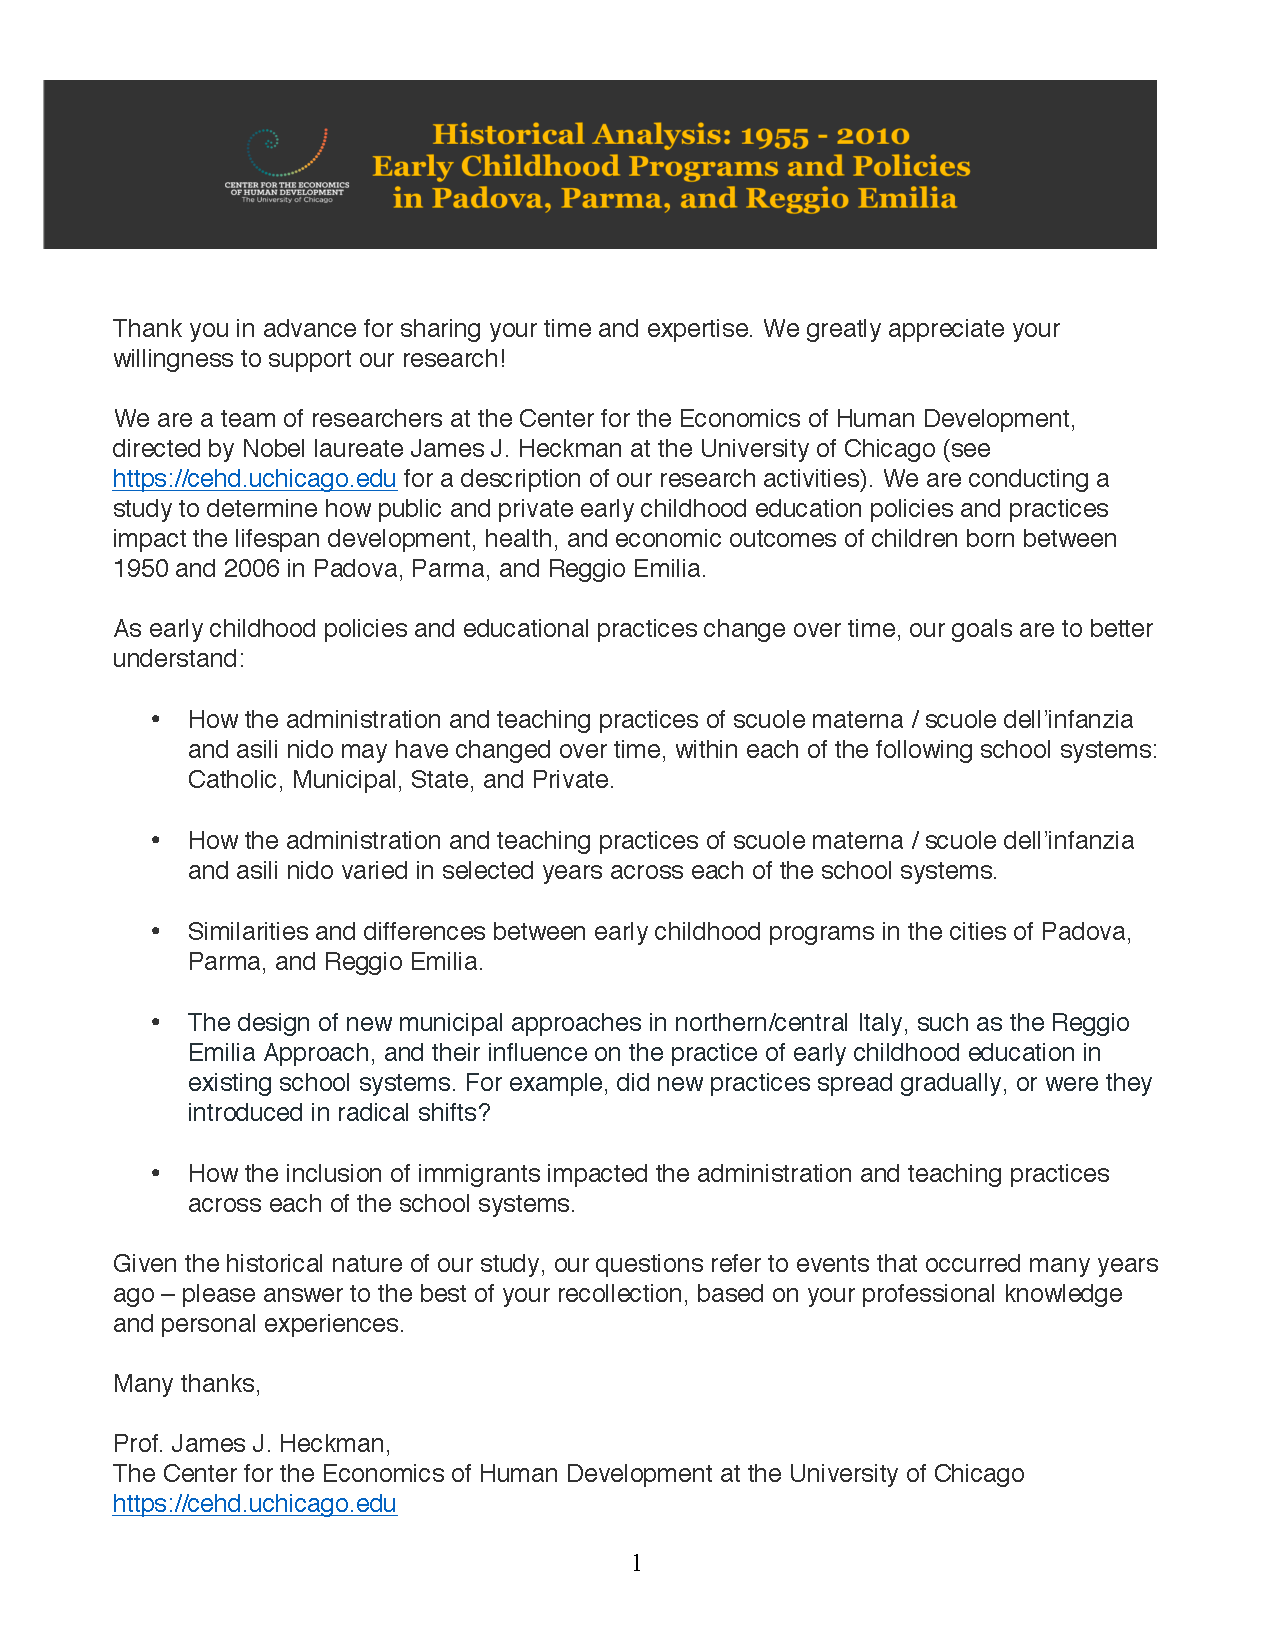
\includepdf[pages=-]{section/CEHD-ECE-Italy_SurveyQuestionnaire-ENGLISH_2016-10-24_sk}